\documentclass{standalone}
\usepackage{tikz}
\usepackage{graphicx}
\usepackage{pgfmath}
\usetikzlibrary{backgrounds,shapes,arrows,positioning,calc,snakes,fit,arrows.meta}
\usepgflibrary{decorations.markings,decorations.text}
\tikzset{>=latex}

\begin{document}

\sffamily

  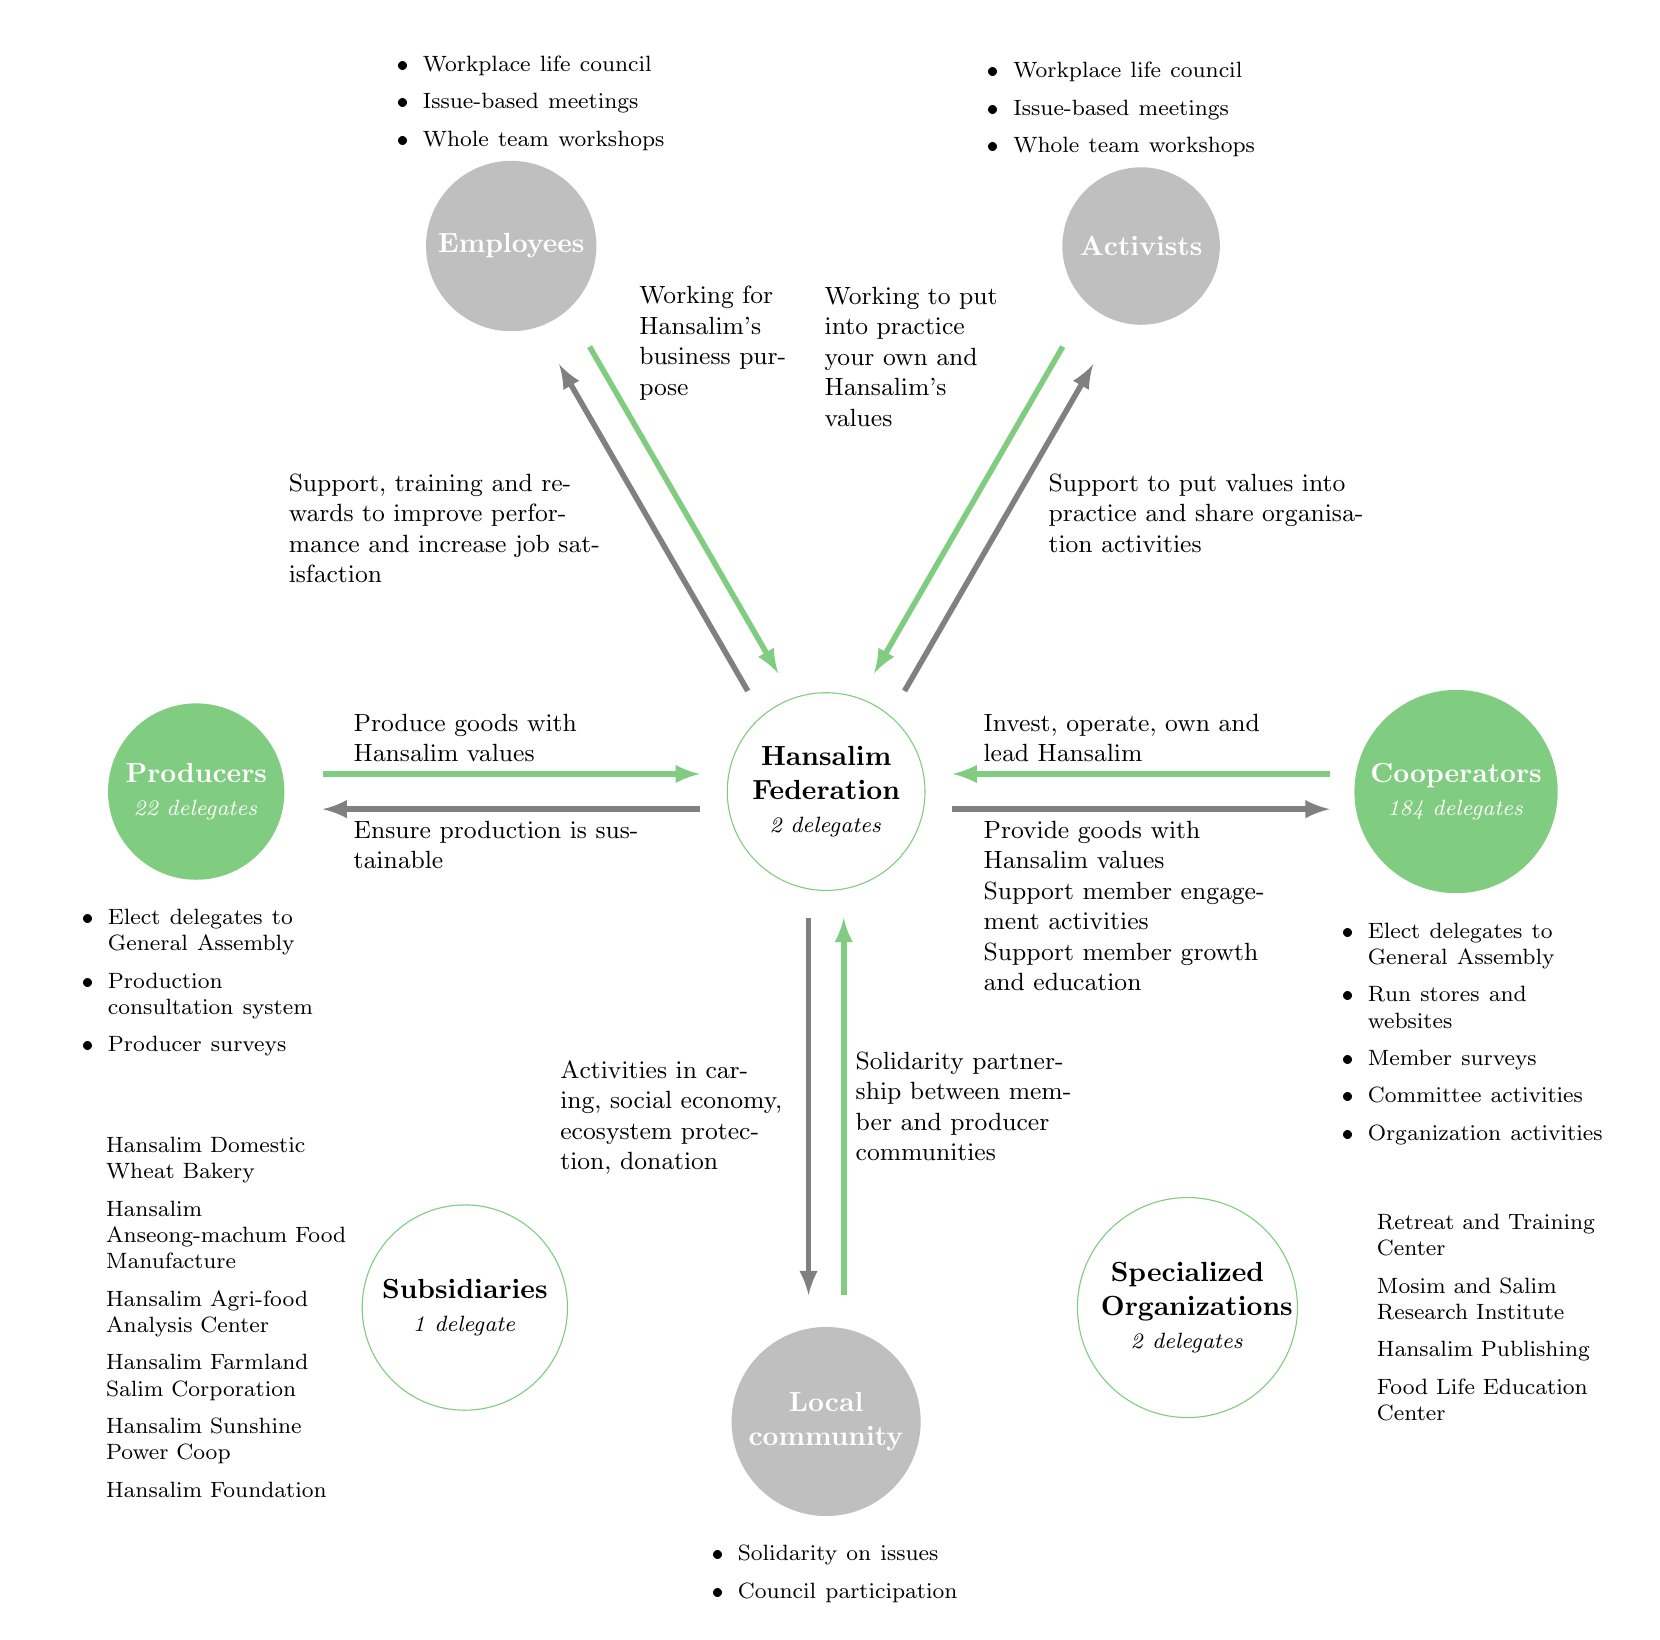
\begin{tikzpicture}

% Angles and Radius
    \def\LevelOne{2}
    \def\LevelTwo{4}
    \def\LevelThree{6}
    \def\LevelFour{8}
    \def\LevelEdge{8.5}
    
    \def\AngleTwelve{90}
    \def\AngleOne{60}
    \def\AngleTwo{30}
    \def\AngleThree{360}
    \def\AngleFour{340}
    \def\AngleFive{305}
    \def\AngleSix{270}
    \def\AngleSeven{235}
    \def\AngleEight{200}
    \def\AngleNine{180}
    \def\AngleTen{150}
    \def\AngleEleven{120}

% Coordinates

    \coordinate (originNode) at (0:0);
    \coordinate (Clock-12) at (\AngleTwelve:\LevelFour);
    \coordinate (Clock-01) at (\AngleOne:\LevelFour);
    \coordinate (Clock-02) at (\AngleTwo:\LevelFour);
    \coordinate (Clock-03) at (\AngleThree:\LevelFour);
    \coordinate (Clock-04) at (\AngleFour:\LevelFour);
    \coordinate (Clock-05) at (\AngleFive:\LevelFour);
    \coordinate (Clock-06) at (\AngleSix:\LevelFour);
    \coordinate (Clock-07) at (\AngleSeven:\LevelFour);
    \coordinate (Clock-08) at (\AngleEight:\LevelFour);
    \coordinate (Clock-09) at (\AngleNine:\LevelFour);
    \coordinate (Clock-10) at (\AngleTen:\LevelFour);
    \coordinate (Clock-11) at (\AngleEleven:\LevelFour);

    \coordinate (Clock-07-5) at ({(\AngleSeven+\AngleEight)/2}:\LevelFour);
    \coordinate (Clock-06-5) at ({(\AngleSix+\AngleSeven)/2}:\LevelFour);
    \coordinate (Clock-05-5) at ({(\AngleFive+\AngleSix)/2}:\LevelFour);
    \coordinate (Clock-04-5) at ({(\AngleFour+\AngleFive)/2}:\LevelFour);

% Colors
    \def\ColGreen{green!60!black!50}
    \def\ColGray{gray!50}
    \def\ColBlack{black!50}

% Stakeholder Nodes
    \node (hansalim) [circle,draw=\ColGreen,minimum width=2.5cm,align=center] at (originNode) {\textbf{Hansalim}\\\textbf{Federation}\\\footnotesize{\textit{2 delegates}}};
    \node (activists) [circle,color=white!100,fill=\ColGray,minimum width=2cm] at (Clock-01) {\textbf{Activists}};
    \node [above,text width=5cm] at (activists.north) {\footnotesize{\begin{itemize}
            \item Workplace life council
            \item Issue-based meetings
            \item Whole team workshops
        \end{itemize}}};    
    \node (cooperators) [circle,color=white!100,fill=\ColGreen,minimum width=2cm,align=center] at (Clock-03) {\textbf{Cooperators}\\\footnotesize{\textit{184 delegates}}};
    \node [below,text width=4cm] at (cooperators.south) {\footnotesize{\begin{itemize}
            \item Elect delegates to General Assembly
            \item Run stores and websites
            \item Member surveys
            \item Committee activities
            \item Organization activities
        \end{itemize}}};
    \node (community) [circle,color=white!100,fill=\ColGray,minimum width=2cm,align=center] at (Clock-06) {\textbf{Local}\\\textbf{community}};
    \node [below,text width=4cm] at (community.south) {\footnotesize{\begin{itemize}
            \item Solidarity on issues
            \item Council participation
        \end{itemize}}}; 
    \node (producers) [circle,color=white!100,fill=\ColGreen,minimum width=2cm,align=center] at (Clock-09) {\textbf{Producers}\\\footnotesize{\textit{22 delegates}}};
    \node [below,text width=4cm] at (producers.south) {\footnotesize{\begin{itemize}
            \item Elect delegates to General Assembly
            \item Production consultation system
            \item Producer surveys
        \end{itemize}}}; 
    \node (employees) [circle,color=white!100,fill=\ColGray,minimum width=2cm] at (Clock-11) {\textbf{Employees}};
    \node [above,text width=4cm] at (employees.north) {\footnotesize{\begin{itemize}
            \item Workplace life council
            \item Issue-based meetings
            \item Whole team workshops
        \end{itemize}}};

    \node (subsidiaries) [circle,draw=\ColGreen,text width=2.2cm,align=center] at (Clock-07) {\textbf{Subsidiaries}\\\footnotesize{\textit{1 delegate}}};
    \node [left,text width=4cm,font=\footnotesize] at (subsidiaries.west) {\begin{itemize}
        \renewcommand\labelitemi{}
            \item Hansalim Domestic Wheat Bakery
            \item Hansalim Anseong-machum Food Manufacture
            \item Hansalim Agri-food Analysis Center
            \item Hansalim Farmland Salim Corporation
            \item Hansalim Sunshine Power Coop
            \item Hansalim Foundation
        \end{itemize}};
    \node (departments) [circle,draw=\ColGreen,text width=2.2cm,align=center] at (Clock-05) {\textbf{Specialized\\Organizations}\\\footnotesize{\textit{2 delegates}}};
    \node [right,text width=4cm,font=\footnotesize] at (departments.east) {\begin{itemize}
        \renewcommand\labelitemi{}
            \item Retreat and Training Center
            \item Mosim and Salim Research Institute
            \item Hansalim Publishing
            \item Food Life Education Center
        \end{itemize}};

% Arrows
% #1 = from node, #2 = to node, #3 = arrow label, #4 = colour, #5 = text width, #6 = anchor, #7 = position, #8 = arrow direction
\def\inArrow(#1,#2,#3,#4,#5,#6,#7,#8){
    \def\fromNode{#1};
    \def\toNode{#2};
        \draw[#4, {#8},
        line width=2pt] ($ (\toNode)!.8! 2:(\fromNode) $) -- ($ (\fromNode)!.8! -2:(\toNode) $) node[text width=#5,pos=#7,anchor=#6,font=\small,color=black!100] {#3};
}

\inArrow(cooperators,hansalim,
        {Invest, operate, own and lead Hansalim},
    \ColGreen,4cm,south,0.5,->)
\inArrow(hansalim,cooperators,
        {Provide goods with Hansalim values\\
        Support member engagement activities\\
        Support member growth and education},
    \ColBlack,4cm,north,0.5,->)

\inArrow(activists,hansalim,
        {Working to put into practice your own and Hansalim’s values},
    \ColGreen,2.2cm,south east,0.28,->)
\inArrow(hansalim,activists,
        {Support to put values into practice and share organisation activities},
    \ColBlack,4cm,north west,0.7,->)

\inArrow(employees,hansalim,
        {Support, training and rewards to improve performance and increase job satisfaction},
    \ColBlack,4cm,north east,0.3,<-)
\inArrow(hansalim,employees,
        {Working for Hansalim’s business purpose},
    \ColGreen,2.2cm,south west,0.8,<-)

\inArrow(hansalim,producers,
        {Produce goods with Hansalim values},
    \ColGreen,4cm,south,0.5,<-)
\inArrow(producers,hansalim,
        {Ensure production is sustainable},
    \ColBlack,4cm,north,0.5,<-)

\inArrow(hansalim,community,
        {Activities in caring, social economy, ecosystem protection, donation},
    \ColBlack,3cm,east,0.53,->)
\inArrow(community,hansalim,
        {Solidarity partnership between member and producer communities},
    \ColGreen,3cm,west,0.5,->)

%    \draw[black!90, {Stealth[inset=0pt, angle=90:4pt]-},
%        line width=1pt] ($ (members)!.8! -5:(hansalim) $) -- ($ (hansalim)!.8! 5:(members) $) node[midway,above,font=\small,color=black!100] {Arrow label};

  \end{tikzpicture}

\end{document}
